\documentclass[12pt,a4paper]{scrartcl}
\usepackage[utf8]{inputenc}
\usepackage{csquotes}
\usepackage[ngerman]{babel}
\usepackage{amsmath}
\usepackage{amsfonts}
\usepackage{amssymb}
\usepackage{graphicx}
\usepackage{gensymb}
\usepackage{float}
\usepackage{microtype}
\usepackage[per-mode = fraction]{siunitx}
\DeclareSIUnit{\bit}{Bit}
\DeclareSIUnit{\chip}{Chip}

\usepackage[backend=biber]{biblatex}
\addbibresource{./sources.bib}
\author{Leon Bentrup}
\title{GPS}
\subtitle{Satellitennavigation}
\begin{document}
\maketitle
\tableofcontents
\newpage
\KOMAoptions{parskip=full}

\section{Vorwort}
\section{Navigation}
Die satellitengestützten Navigationssysteme, die wir heute verwenden, benutzen das gleiche grundlegende Prinzip, das auch schon die Seefahrer der Antike eingesetzt haben, als sie sich an den Sternen orientiert haben.

Man verwendet Objekte im Weltall, deren Position man kennt, um die eigene Position auf der Erde zu bestimmen.

\subsection{Sextant}
Mit einem Sextanten bestimmt man den eigenen Breitengrad mit Hilfe von drei Sternen.
Zuerst muss der Höhenwinkel von drei bekannten Sternen gemessen werden. Der Höhenwinkel ist der Winkel zwischen Horizont, dem Betrachter und dem Stern.
Danach entnimmt man aus einem Nautischen Almanach die Koordinaten der angepeilten Sterne. Aus diesen drei Messungen ergeben sich dann drei Kegel. Sie sind durch den Stern als Spitze und durch den gemessenen Höhenwinkel als Winkel zwischen Boden und Mantelfläche des Kegels genau definiert. Die Kanten zwischen Boden und Mantel schneiden sich in einem Punkt. Dieser Schnittpunkt ist die eigene Position.

\begin{figure}[H]
\centering
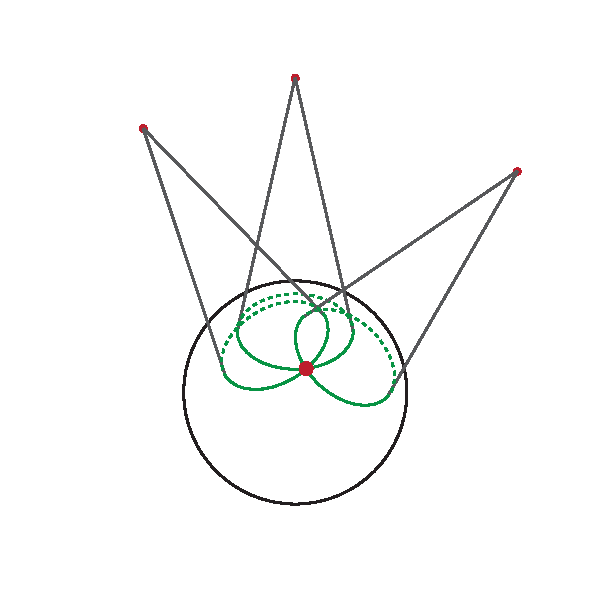
\includegraphics[width=0.7\textwidth]{img/earth_cones.pdf}
\caption{Positionsbestimmung anhand der Höhenwinkel von drei Sternen}
\end{figure}

\subsection{Koordinatensystem der Erde}
Um eine Position auf der Erde anzugeben verwendet man kein „normales“ Koordinatensystem, mit X-, Y- und Z-Koordinaten. Denn da die Erden eine Kugel (Ellipsoid) ist, und die Oberfläche gekrümmt ist, kann man mit solch einem Koordinatensystem nicht einfach rechnen. Würde man die Koordinaten für zwei Punkte am Boden und an der Spitze eines Turms angeben, müsste man dafür nicht nur eine Koordinate anpassen, sondern wahrscheinlich alle 3, um von einem Punkt auf den anderen zu kommen.

Deshalb verwendet man in der Navigation ein System von Längengraden, Breitengraden und der Höhe über dem Meeresspiegel.

\paragraph{Breitengrade} Die Breitengrade verlaufen parallel zum Äquator der Erde. Sie reichen dabei von 90\degree{} Nord (oder nur 90\degree), der Nordpol über 0\degree, der Äquator bis 90\degree{} Süd (oder -90\degree), der Südpol. Ein Breitengrad ist also der Winkel zwischen Äquator, Erdmittelpunkt und dem zugehörigen Punkt auf der Erdoberfläche.

\paragraph{Längengrade}
Die Längengrade verlaufen senkrecht zu den Breitengraden. Ein Längengrad beschreibt also eine Linie vom Nordpol zum Südpol. Der Nullmeridian (0\degree{}) wurde durch internationale Vereinbarungen auf das \emph{Royal Greenwich Observatory} in England gelegt. Von dort aus misst man von 180\degree{} West bis 180\degree{} Ost, um die Erde zu umspannen.

\begin{figure}
\centering
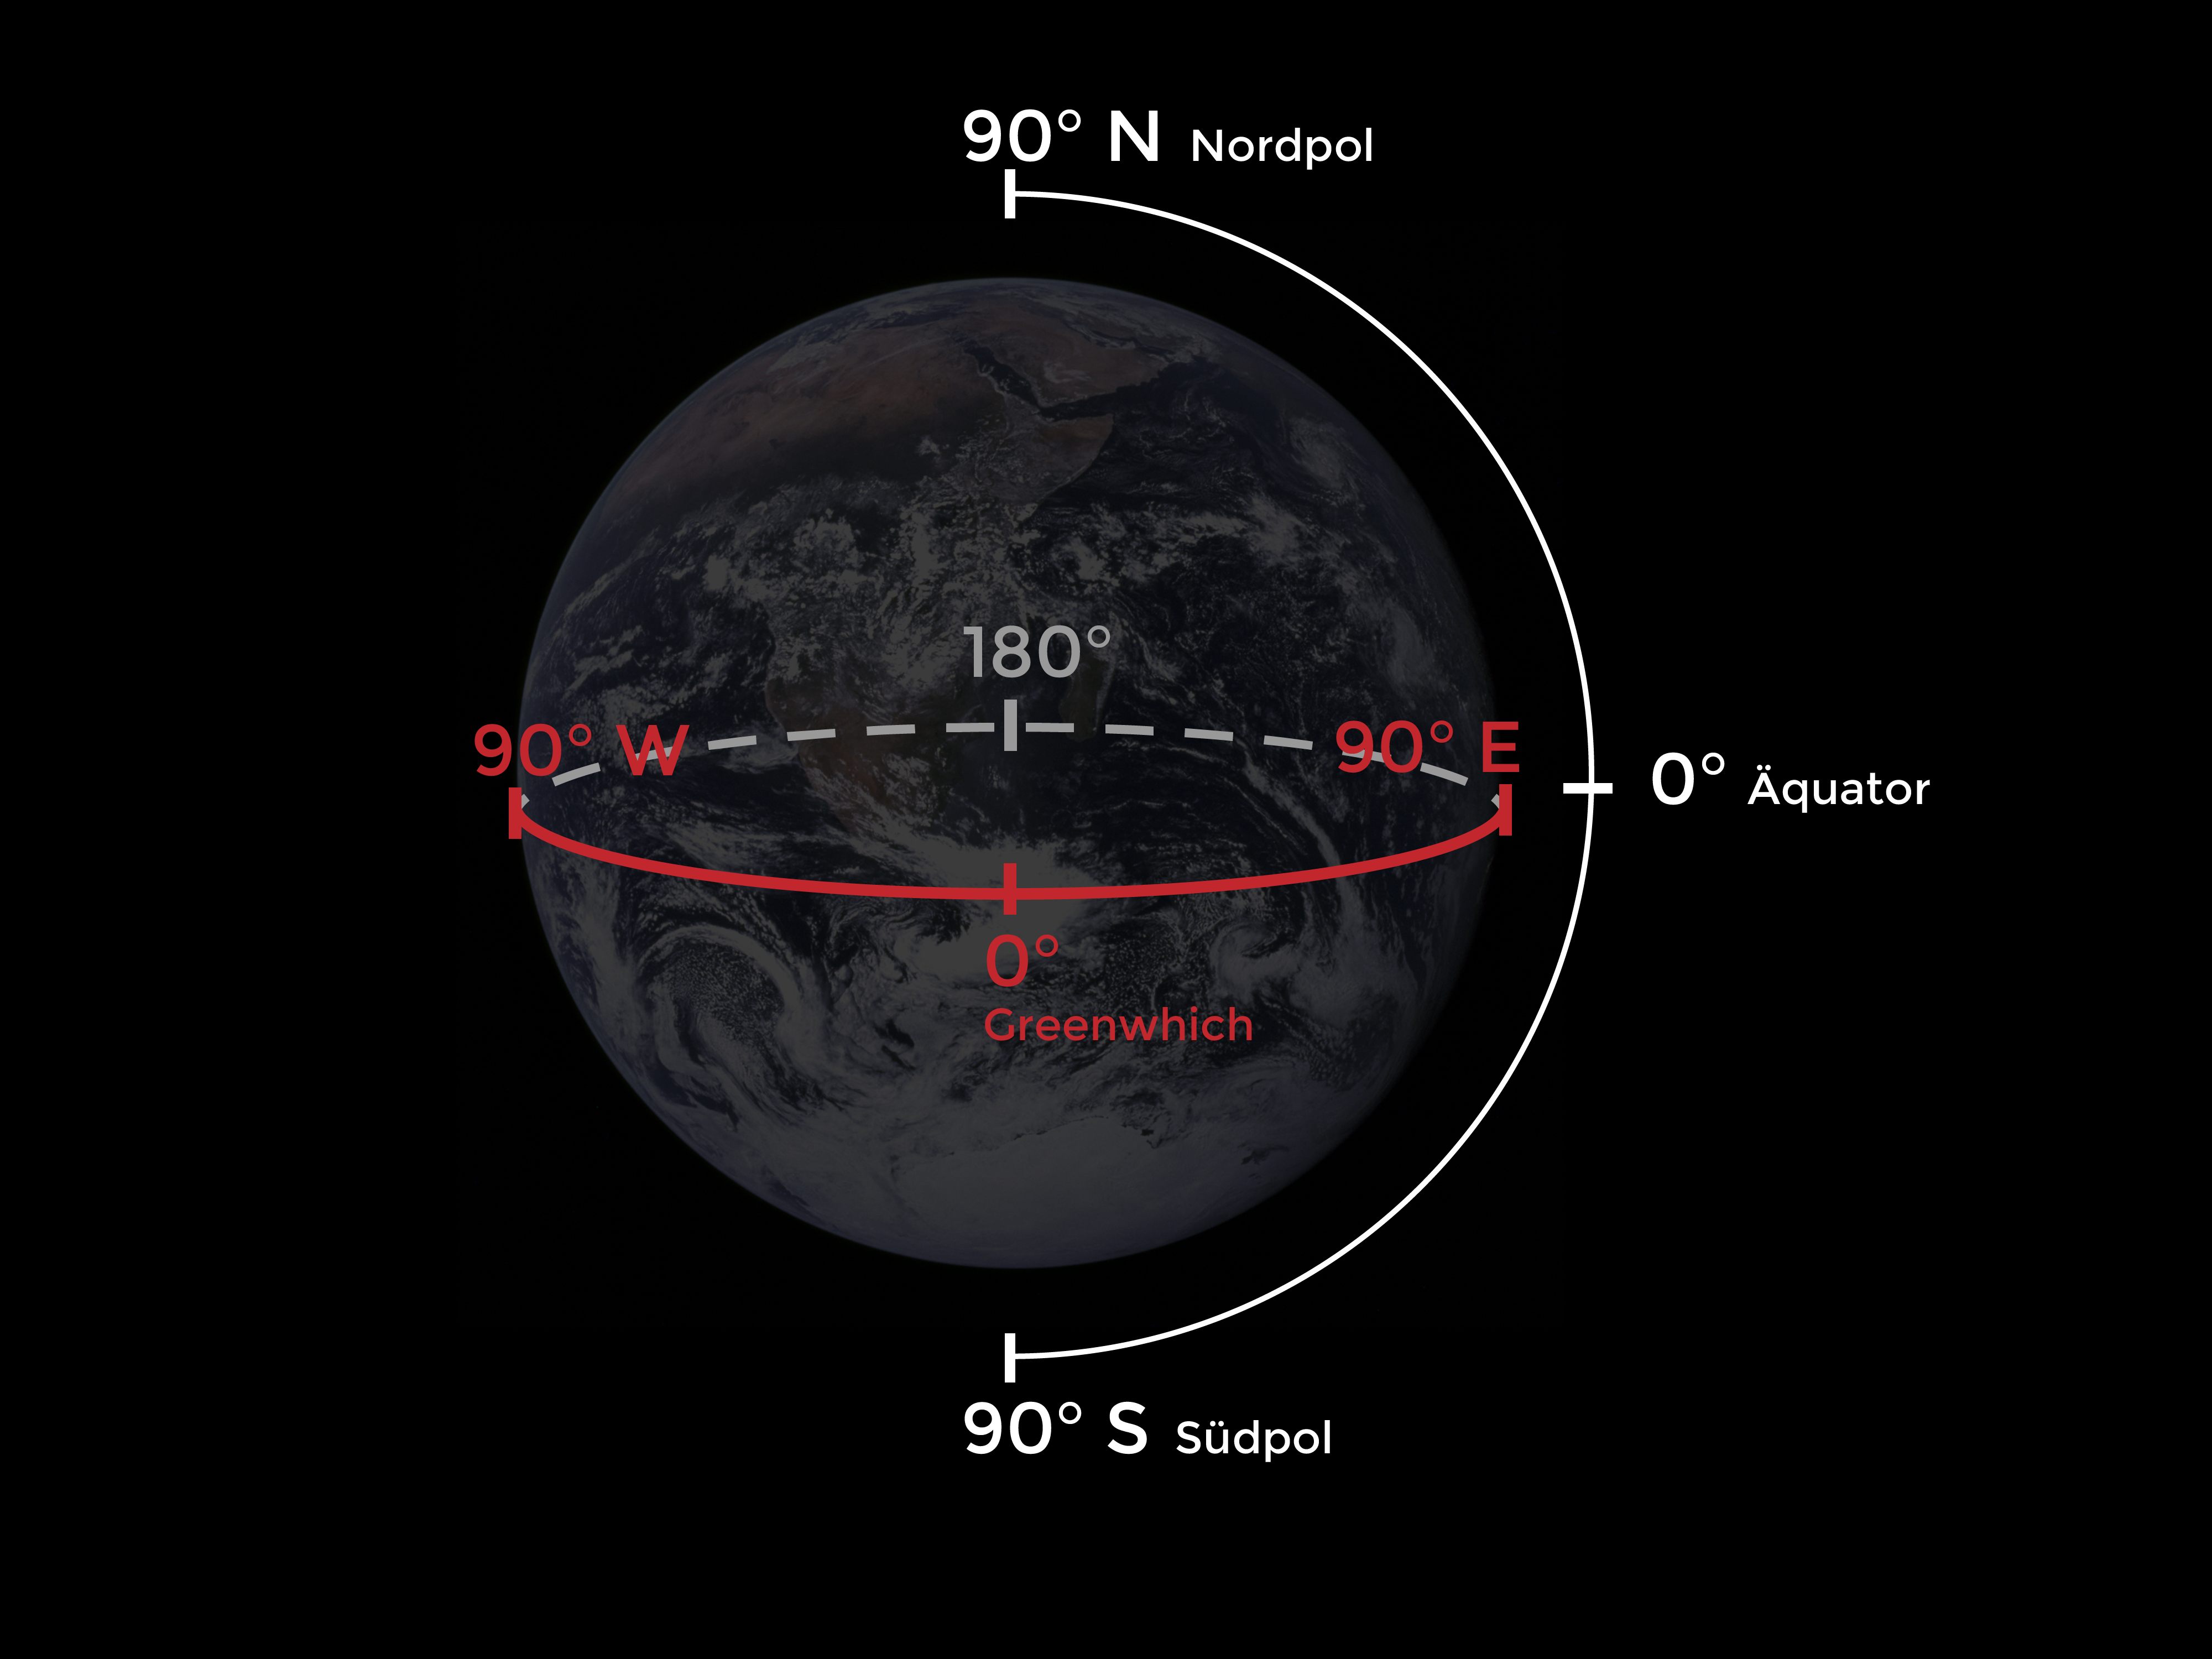
\includegraphics[width=0.7\textwidth]{img/latlong-01.png}
\caption{Längen- und Breitengrade der Erde}
\end{figure}

\paragraph{Höhe}
In der Navigation finden Höhenangaben eigentlich nur geringe Beachtung, denn Längen- und Breitengrade reichen aus, um einen Punkt \emph{auf} der Erd\emph{oberfläche} anzugeben. Trotzdem ist die Höhe notwendig, um mittels Längen- und Breitengraden einen Punkt im dreidimensionalen Raum eindeutig zu definieren. (Auch bei der Navigation in Flugzeugen ist sie natürlich wichtig.) Die Höhe wird in einer Längeneinheit über einem definierten Nullpunkt angegeben. Für die Höhenmessung gibt es allerdings viele verschiedene Systeme, und verschiedene Länder verwenden verschiedene Nullpunkte (z.B. „Normalhöhennull“ in Deutschland).

\section{GPS-System}

\subsection{Segmente}
Das GPS-System wird in drei Segmente eingeteilt. Diese sind:
\begin{itemize}
\item Das Space Segment, die Satelliten im Weltall
\item Das Control Segment, mehrere weltweit verteilte Bodenstationen zur Überwachung und Steuerung der GPS-Satelliten
\item Das User Segment, die Nutzer des GPS-Systems, also die GPS-Empfänger
\end{itemize}
\cite{gpsgov_segments}

\subsection{GPS-Satellit}
Die GPS-Satelliten stellen im GPS-System das dar, was früher die Sterne waren. Sie sind die Fixpunkte, deren Position bekannt ist.

Ein GPS-Satellit umkreist die Erde in einer Höhe von ca. \SI{26600}{\kilo\meter}, gemessen zum Erdmittelpunkt.
Mit dem 3. Keplerschen Gesetz \eqref{eq:kepler3} kann man daraus die Umlaufzeit $T$ berechnen.

\begin{equation}
\label{eq:kepler3}
T^2 = \frac{4 \pi^2}{G (M + m)} \cdot a^3
\end{equation}
\cite{wiki_kepler}

Die Masse des Satelliten $m$ ist dabei im Vergleich zur Erdmasse vernachlässigbar.

\begin{align*}
a &= \SI{2.66e6}{\meter} && \text{Abstand des Satelliten}\\
M &= \SI{5.97219e24}{\kilo\gram} && \text{Masse der Erde}\\
G &= \SI{6.67408e-11}{\cubic\meter\per\kilo\gram\per\square\second} && \text{Gravitationskonstante} \\
T^2 &= \frac{4 \pi^2}{G M} \cdot a^3 \\
T &= \sqrt{\frac{4 \pi^2}{\SI{6.67408e-11}{\cubic\meter\per\kilo\gram\per\square\second} \cdot \SI{5.97219e24}{\kilo\gram}} \cdot (\SI{2.66e6}{\meter})^3} \\
T &= \SI{11.9932}{\hour} && \text{11 Stunden und 58 Minuten}
\end{align*}

Die Position der GPS-Satelliten ist also von der Erde aus gesehen nicht immer gleich, sondern sie Umkreisen die Erde zwei mal pro Tag.

Das Herzstück jedes GPS-Satelliten ist eine sehr präzise Atomuhr. Sie ist mit den Atomuhren der anderen Satelliten synchronisiert und liefert die GPS-Zeit, die Grundlage für das GPS-System.

Weitere Geräte sind für die Verarbeitung der Uhrzeit, das eigentliche Senden des GPS-Signals und die Kommunikation mit Bodenstationen zuständig.

Die GPS-Satelliten werden über Solarzellen mit Strom versorgt. Deshalb müssen sie sehr energieeffizient sein. Die knappe Stromzufuhr ermöglicht außerdem keine große Sendeleistung für das GPS-Signal. Das Empfangen der Signale ist deshalb in der Praxis sehr schwierig. In Gebäuden oder unter Wasser ist es meist gar nicht möglich.

\subsection{Konstellation}
Für eine Positionsbestimmung müssen die Signale von mindestens 4 Satelliten empfangen werden (siehe \ref{sec:positioning}). Zusätzliche Satelliten erhöhen die Genauigkeit. Damit dies an jedem Punkt auf der Erde gewährleistet ist, muss es genug GPS-Satelliten geben, die richtig um die Erde verteilt sind.

Die Anordnung der Satelliten wird \emph{Konstellation} genannt. Die GPS-Konstellation besteht aus mindestens 24 Satelliten, die auf 6 kreisförmigen Ebenen mit je 4 Satelliten verteilt sind.

Aktuell sind 30 funktionierende GPS-Satelliten im Weltall. Von den meisten Punkten der Erde aus kann man die Signale von 9 bis 11 Satelliten empfangen.

\section{GPS-Signal}
GPS-Satelliten senden Signale auf verschiedenen Frequenzen gleichzeitig. Diese Bänder werden $L_1$ bis $L_5$ genannt. Das für Zivile Empfänger wichtigste Signal, das C/A-Signal, wird über das $L_1$-Band mit der Frequenz
\begin{equation}
f_{L_1} = \SI{1.57542}{\giga\hertz} \nonumber
\end{equation}
übertragen.

Untereinander unterscheiden sich die Frequenzen, die von den GPS-Satelliten verwendet werden jedoch nicht. Das bedeutet, dass der GPS-Empfänger Signale von bis zu 12 Satelliten auf einer Frequenz unterscheiden muss.

\subsection{CDMA}

Um das zu erreichen wird eine Technik namens CDMA angewendet.
CDMA steht für \emph{Code Division Multiple Access}. Es beschreibt ein Verfahren, wobei man mit Hilfe von Codes die gleichzeitige Übertragung mehrerer Signale auf einer Frequenz ermöglicht.

Dazu benötigt jeder Sender auf der jeweiligen Frequenz einen eigenen Code. Im Grunde genommen eine Folge von 1 und 0, die den Sender kennzeichnet. Im Fall von GPS ist dies ein pseudo-zufälliges Rauschen, welches sich nach \SI{1023}{\chip} wiederholt. Ein Chip ist ein Symbol des Codes, also eine 1 oder eine 0. Man verwendet den Begriff Chip statt Bit, da es sich beim Code nicht um wirkliche Informationen handelt. Dieser Code wird C/A-Code genannt.

Der Code wird mit \SI{1023}{\mega\chip\per\second} übertragen, was bedeutet, dass er sich jeweils nach 1 Millisekunde wiederholt.
Die Nutzdaten werden deutlich langsamer, mit \SI{50}{\bit\per\second} übertragen. Dann werden Code und Nutzdaten mit einem exklusiven Oder (XOR) verknüpft.

Ein exklusives Oder verknüpft die beiden Eingänge A und B zu einem Ausgang. Das XOR ist dann war, wenn A oder B wahr ist, aber nicht, wenn A und B wahr sind.

\begin{center}
\begin{tabular}{cc|c}
\textbf{$A$} & \textbf{$B$} & \textbf{$A\oplus B$} \\
0 & 0 & 0 \\
1 & 0 & 1 \\
0 & 1 & 1 \\
1 & 1 & 0 \\
\end{tabular}
\end{center}

Zeichnet man die Daten entlang einer Zeitachse, erhält man folgendes Bild:

\begin{figure}[H]
\centering
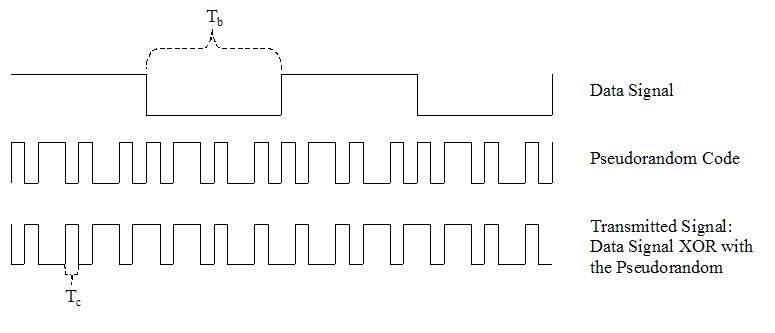
\includegraphics[width=0.9\textwidth]{img/Generation_of_CDMA.jpg}
\caption{Visualisierung des CDMA-Verfahren\cite{commons_cdma}}
\label{fig:cdma}
\end{figure}

% TODO: Rephrase encouraged
Dort kann man sehen, dass das übertragene Signal genau dem Code entspricht, wenn das Datensignal 0 ist, und dass es dem negierten (umgekehrten) Code entspricht, wenn das Datensignal 1 ist.

\subsection{Satellitencodes}

Der C/A Code jedes Satelliten wird mit einem Pseudozufallsgenerator erzeugt. Das bedeutet, dass die Ausgabe zufällig aussieht, das Gerät aber bei gleichen Anfangsbedingungen auch wieder die gleiche Zufallsfolge erzeugt. Jeder GPS-Empfänger kann also den C/A-Code selbst generieren. Über zwei Parameter im Algorithmus dieses Zufallsgenerators wird ausgewählt, für welchen Satelliten der Code erzeugt werden soll. Die Codes sind so ausgewählt, dass das Unterscheiden der verschiedenen Satelliten für den Empfänger möglichst einfach ist (siehe \ref{sec:correlation}).

(Meine Implementierung des Zufallsgenerators in der Programmiersprache Python befindet sich im Anhang.)

\subsection{Modulation}

Modulation ist ein Verfahren, um Daten mittels Funkwellen zu „kodieren“.
Wenn man nur eine Funkwelle (mit einer bestimmten Frequenz) sendet, werden so noch keine Daten übertragen. Dies geschieht erst, wenn bestimmte Eigenschaften dieser sogenannten Trägerwelle verändert werden.

Ein sehr simples Beispiel für eine solche Modulation ist die \emph{Amplitudenmodulation}, die beim Mittelwellenradio zum Einsatz kommt. Dabei wird die Amplitude der Trägerwelle variiert und so Daten übertragen. Beim Radio wird so die Amplitude der Trägerwelle an die Auslenkung der Schallwelle angepasst. Graphisch sieht dies so aus:

\begin{figure}[H]
\centering
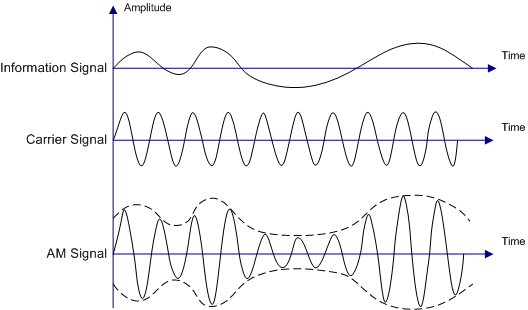
\includegraphics[width=0.9\textwidth]{img/Illustration_of_Amplitude_Modulation.png}
\caption{Visualisierung der Amplitudenmodulation\cite{commons_am}}
\label{fig:am}
\end{figure}

In der Grafik kann man schon sehen, dass die Frequenz des Trägersignals deutlich größer sein muss, als die des Nutzdatensignals, da es sonst zu starken Qualitätsverlusten kommt.

Es gibt sehr viele verschiedene Verfahren zur Modulation. Sie unterscheiden sich z.B. in der Fehleranfälligkeit (manche Reagieren auf Störungen der Übertragung heftiger als andere). Es gibt kein \emph{bestes} Modulationsverfahren, es kommt immer auf den Einsatzzweck an. Mit manchen Verfahren kann man nur digitale Signale übertragen, mit anderen auch analoge.

Die Daten, die ein GPS-Satellit sendet werden auf eine Trägerwelle (mit der Frequenz des $L_1$-Bands) mit dem \emph{Binary Phase-Shift Keying}, kurz BPSK-Verfahren moduliert.
Bei diesem Verfahren wird die sinusförmige Trägerwelle in ihrer Phase um $\frac{\lambda}{2}$ vor oder zurück verschoben, wenn in den Nutzdaten ein Wechsel von 1 zu 0 oder von 0 zu 1 vorliegt.

\begin{figure}[H]
\centering
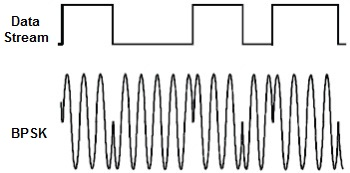
\includegraphics[width=0.7\textwidth]{img/bpsk.jpg}
\caption{Visualisierung des BPSK-Verfahrens\cite{evalidate_bpsk}}
\label{fig:bpsk}
\end{figure}

\subsection{Navigationsnachricht}
Die Informationen, die über das GPS-Signal übertragen werden nennt man \emph{Navigationsnachricht}. Die Navigationsnachricht enthält:
\begin{itemize}
\item Nummer der GPS-Woche (seit 22. August 1999)
\item Zeit, die seit Beginn der Woche vergangen ist, in 6s-Schritten
\item Abweichung der Satellitenzeit von der GPS-Systemzeit
\item Informationen über die Umlaufbahn des eigenen und anderer Satelliten (Ephemeriden)
\item Korrekturdaten für Verzerrung durch die Ionosphäre
\item Abweichung der GPS-Systemzeit von der UTC-Zeit (die GPS-Zeit kennt keine Schaltsekunden)
\item Informationen über den Zustand der GPS-Satelliten
\end{itemize}
\cite{infotip_gps}

Die Daten sind dabei in 25 Frames aufgeteilt, die wieder aus 5 Subframes bestehen. Ein Subframe fasst 10 Wörter mit je \SI{30}{\bit}.

Die Navigationsnachricht wird mit \SI{50}{\bit\per\second} übertragen.
Ein Subframe benötigt also \SI{6}{\second} für die Übertragung, ein Frame \SI{30}{\second}. Bis die vollständige Navigationsnachricht übertragen ist, vergehen \SI{12.5}{\minute}.

Das erste Wort jedes Subframes ist das Telemetrie-Wort (TLM). Es enthält das Präambel, eine definierte Reihenfolge von 1 und 0, die ein GPS-Empfänger benutzt, um den Beginn des Subframes zu erkennen.  Darauf folgt das Hand Over Word (HOW), dass die Zeit seit Beginn der Woche zählt. Sie wird in \SI{6}{\second}-Schritten gezählt, der Länge eines Subframes. Die verbleibenden 8 Wörter eines Subframes sind dann für die eigentliche Datenübertragung.

\begin{figure}[H]
\centering
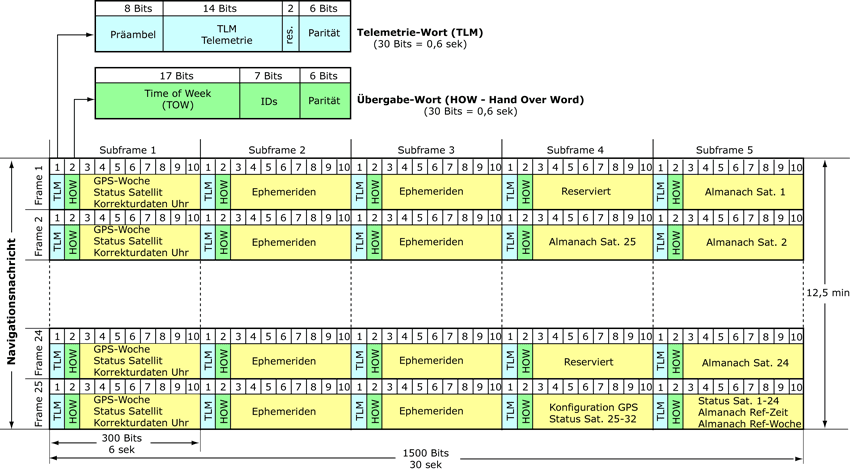
\includegraphics[width=\textwidth]{img/navigation_message.png}
\caption{Die GPS-Navigationsnachricht\cite{infotip_gps}}
\label{fig:nm}
\end{figure}

\section{GPS-Empfänger}
GPS-Empfänger gibt es in verschiedenen Modellen. Von kleinsten Modulen, die in Smartphones eingebaut werden, bis zu großen professionellen GPS-Empfängern für die Vermessung von Grundstücken.

Ein GPS-Empfänger benötigt mindestens folgende Komponenten:

\paragraph{Antenne}
In GPS-Empfängern kommen aktive Antennen zum Einsatz, die direkt an der Antenne einen Verstärker angebracht haben. Das verringert Störeinflüsse, die sonst über die Verbindung zwischen Antenne und Verstärker entstehen würden. Außerdem enthalten GPS-Empfänger noch Elektronik zum Filtern, Verstärken und Demodulieren des empfangenen Signals.

\paragraph{DSP-Chip}
Der DSP-Chip übernimmt die zeitkritischen und anspruchsvollen Aufgaben, die zum Bestimmen der Laufzeiten zu den Satelliten und daraus der Position des Empfängers notwendig sind.

\paragraph{Uhr}
Ein GPS-Empfänger benötigt eine genaue Uhr, z.B. eine Quarz-Uhr. Sie ist zum einen der Zeitgeber für das Auswerten des GPS-Signals und sie behält die Zeit, wenn der GPS-Empfänger ausgeschaltet ist, was später einen Warmstart ermöglicht.

\paragraph{Mikrocontroller}
Weniger anspruchsvolle Berechnungen, wie z.B. das Umrechnen von Koordinaten in ein anderes Format oder die Kommunikation mit internem Speicher, Display und angeschlossenen Geräten, übernimmt ein Mikrocontroller.

\section{GPS-Fix}
Die Aufgabe, die ein GPS-Empfänger bewältigen muss ist keine leichte.
Denn durch die sehr kleine Sendeleistung der GPS-Satelliten und deren große Entfernung ist das GPS-Signal auf der Erde so schwach, dass es im Hintergrundrauschen „untergeht“. Zusätzlich dazu überlagern sich auch noch die Signale mehrerer Satelliten. Dementsprechend ist das Aufbereiten und Auswerten des GPS-Signals sehr kompliziert. Deshalb wird der Prozess im Nachfolgenden etwas vereinfacht dargestellt.

\subsection{Autokorrelation}
\label{sec:correlation}
Zunächst muss der GPS-Empfänger die Zeit feststellen, zu der ein von ihm empfangenes Signal gesendet wurde. Er beginnt damit, für einen Satelliten den C/A-Code zu generieren. Diesen Code vergleicht der Empfänger dann mit dem empfangenen Signal. Der Algorithmus, der dazu verwendet wird heißt Autokorrelation.

Dazu werden die empfangenen Daten und der interne C/A-Code mit einem UND verknüpft. Danach wird die Summe aus den so entstandenen Werten gebildet. Dieser Wert muss maximiert werden. Dazu verschiebt der GPS-Empfänger den generierten C/A-Code. Außerdem muss noch die Frequenz des Empfängers um $\pm \SI{6}{\kilo\hertz}$ angepasst werden. Denn die Satelliten bewegen sich zum Empfänger hin, oder von ihm weg. Wegen des Doppler-Effektes verändert sich dann die Frequenz der GPS-Signale aus Sicht des Empfängers.

Findet sich auch nach Ausprobieren dieser Verschiebungen keine Kombination, bei der die Autokorrelation einen hohen Wert ergibt, handelt es sich bei dem vom GPS-Empfänger generierten C/A-Code um einen Code, der von keinem Satelliten in „Sichtweite“ verwendet wird.

\begin{figure}[H]
\centering
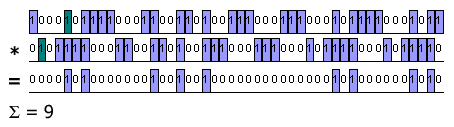
\includegraphics[width=0.7\textwidth]{img/ac_9.png}
\caption{Autokorrelation bei verschobenem Signal\cite{kowoma_signalv}}
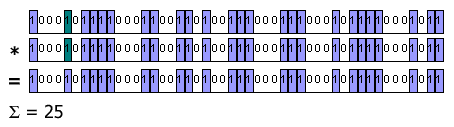
\includegraphics[width=0.7\textwidth]{img/ac_25.png}
\caption{Autokorrelation bei deckendem Signal\cite{kowoma_signalv}}
\label{fig:ac}
\end{figure}

Durch diese Korrelation ist es zum Einen möglich, die Signale verschiedener Satelliten zu unterscheiden, obwohl sich diese überlagern. Außerdem kann so die Sendezeit des Signals bestimmt werden:

Wenn der Empfänger das Signal korreliert hat, kennt er die GPS-Zeit mit $$t_1 = n\cdot\SI{1}{\milli\second} + c; c<\SI{1}{\milli\second}$$ wobei ihm c jetzt bekannt ist, n jedoch nicht. Das folgt daraus, dass sich der C/A-Code jede Millisekunde wiederholt.

\subsection{Sendezeitbestimmung}
Als nächstes sucht der GPS-Empfänger nach einem Bitwechsel in der GPS-Nachricht. Hat er diesen gefunden und zählt die Anzahl der kompletten C/A-Codes, die dabei vergangen sind, kann der GPS-Empfänger die GPS-Zeit mit der Genauigkeit  $$t_1 = n\cdot\SI{20}{\milli\second} + c; c<\SI{20}{\milli\second}$$ bestimmen.

Als nächstes muss nach einem Präambel in der Navigationsnachricht gesucht werden. Das Präambel ist die Bitfolge \texttt{10001011}. Hat der GPS-Empfänger sie gefunden muss er dem Subframe, in dem dieses Präambel enthalten ist die ID entnehmen. Diese ID zeigt, um das wievielte Subframe im Frame es sich handelt. Durch zurückrechnen lässt sich $t_1$ nun mit $$t_1 = n\cdot\SI{6}{\second} + c; c<\SI{6}{\second}$$ bestimmen.

Danach kann aus dem Hand Over Word des Subframes die Zahl der \SI{6}{\second}-Schritte seit Beginn der GPS-Woche gelesen werden. $$t_1 = n\cdot\SI{7}{\day} + c; c<\SI{7}{\day}$$

Schließlich muss der GPS-Empfänger auf das erste Subframe eines Frames warten, dort steht die aktuelle GPS-Woche. Damit ist die GPS-Systemzeit eindeutig bestimmt.

Dieser Vorgang muss mit allen empfangenen Signalen durchgeführt werden.

\subsection{Empfangen der Bahndaten}
Nach der Autokorrelation können alle Signale empfangen werden. Der GPS-Empfänger kann dann die Nutzdaten herunterladen. In diesen Nutzdaten sind die Informationen enthalten, die der GPS-Empfänger braucht, um die aktuelle Position des GPS-Satelliten zu bestimmen. Der GPS-Empfänger bestimmt dann die Positionen der Satelliten, von denen er Signale empfängt.

\subsection{Positionsbestimmung}
\label{sec:positioning}
Dann hat der GPS-Empfänger alle Informationen zusammen, um die eigene Position zu bestimmen. Insgesamt benötigt der GPS-Empfänger die Signale von 4 Satelliten, um eine Positionsbestimmung durchzuführen.

\begin{itemize}
\item Die Position des GPS-Satelliten. $x_i,y_i,z_i$
\item Die Sendezeit des Satelliten. $t_i$
\end{itemize}

Dann kann er für jeden GPS-Satelliten eine Gleichung wie \eqref{eq:gps} aufstellen.
\begin{equation}
\label{eq:gps}
(x_i - x_0)^2 + (y_i - y_0)^2 + (z_i - z_0)^2 = (c\cdot(t_0-t_i))^2
\end{equation}
Dabei ist $x_0,y_0,z_0$ die Position des GPS-Empfängers. $t_0$ ist die aktuelle GPS-Systemzeit, zu dem Zeitpunkt zu dem die Signale empfangen werden. Die Differenz $t_0-t_i$ ist also die Laufzeit des Signals von Satellit zum Empfänger. Mit der Lichtgeschwindigkeit $c$ ergibt sich dann die Entfernung des Empfängers zum Satelliten $c\cdot (t_0-t_i)$. Diese Entfernung ist gleich dem Betrag des Vektors vom Satellit zum Empfänger, wie auf der linken Seite der Gleichung steht.

Für die Satelliten 1-4 ergibt sich dann das Gleichungssystem
\begin{align*}
(x_1 - x_0)^2 + (y_1 - y_0)^2 + (z_1 - z_0)^2 = (c\cdot(t_0-t_1))^2 \\
(x_2 - x_0)^2 + (y_2 - y_0)^2 + (z_2 - z_0)^2 = (c\cdot(t_0-t_2))^2 \\
(x_3 - x_0)^2 + (y_3 - y_0)^2 + (z_3 - z_0)^2 = (c\cdot(t_0-t_3))^2 \\
(x_4 - x_0)^2 + (y_4 - y_0)^2 + (z_4 - z_0)^2 = (c\cdot(t_0-t_4))^2 \\
\end{align*}
Dieses Gleichungssystem mit 4 Gleichungen und 4 Unbekannten kann der GPS-Empfänger dann nach $x_0,y_0,z_0,t_0$ lösen. Er erhält die eigene Position und zusätzlich die sehr exakte GPS-Systemzeit $t_0$, die mit Korrekturdaten aus der Navigationsnachricht in die aktuelle Uhrzeit umgerechnet werden kann.

Diese Berechnungen werden im GPS-Empfänger normalerweise in einem kartesischen Koordinatensystem durchgeführt (3 Achsen, die orthogonal zueinander Stehen). Die ermittelte Position muss also anschließend noch in das Längen- und Breitengradsystem umgerechnet werden.

In der Praxis kann dieses Gleichungssystem natürlich nicht einfach „gelöst“ werden. Durch Ungenauigkeiten gibt es keine exakte Lösung. Stattdessen muss der GPS-Empfänger nach der bestmöglichen Lösung suchen. Es gibt in den meisten Fällen auch zwei reele Lösungen des Gleichungssystems. Eine Lösung scheidet aber immer als unrealistisch aus, weil entweder die GPS-Systemzeit $t_0$ vor der Sendezeit liegt, oder die Position oberhalb der GPS-Satelliten ist.

Außerdem würden hiery noch Korrekturen für Verzerrungen durch die Erdathmosphäre durchgeführt werden. Die dafür benötigten Daten sind ebenfalls in der Navigationsnachricht enthalten.

\subsection{Kalt-, Warm- und Heißstart}
Der gesamte beschriebene Vorgang wird als ein Kaltstart bezeichnet. Er muss durchgeführt werden, wenn der GPS-Empfänger gar keine Informationen über die GPS-Satelliten hat, oder diese veraltet sind. Der Kaltstart kann je nach Zahl der verfügbaren GPS-Satelliten und deren Signalstärke mehrere Minuten dauern. Bei älteren GPS-Empfängern bis zu 20 Minuten.

Deshalb speichert ein GPS-Empfänger Informationen wie die letzte bekannte Position, und die Bahndaten der Satelliten, und behält diese nach dem Ausschalten. Hat sich der GPS-Empfänger seit dem Ausschalten nicht viel bewegt und die gespeicherten Informationen sind noch aktuell, kann ein Warmstart durchgeführt werden. Dann weiß der GPS-Empfänger schon im Voraus, von welchen Satelliten er Signale empfangen kann, und kennt deren ungefähre Bahndaten. Das spart bei der Autokorrelation Zeit, da weniger C/A-Codes ausprobiert werden müssen. Ein Warmstart dauert maximal 45 Sekunden.

Sind noch genaue Bahninformationen vorhanden kann ein Heißstart durchgeführt werden. Dies ist dann der Fall, wenn der Empfang kurz abgerissen ist. Wenn der GPS-Empfänger sich nicht bewegt hat, sind die Daten bis zu 6 Stunden lang aktuell genug für einen Heißstart. Das Bestimmen der Position dauert dann nur wenige Sekunden.

\section{Genauigkeit von GPS}
\label{sec:accuracy}

Bevor die künstliche Verschlechterung des zivilen GPS-Signals, die \emph{Selective Availability} (S/A), abgeschaltet wurde (siehe \ref{sec:history}), konnte man mit zivilen GPS-Empfängern nur Genauigkeiten im \SI{100}{\meter}-Bereich erreichen. Nach der Abschaltung von S/A im Mai 2000, waren alle GPS-Empfänger in der Lage, die Position auf etwa \SI{10}{m} genau zu ermitteln.

Der größte noch verbleibende Störfaktor ist die Ionosphäre der Erde. Die Ionosphäre enthält viele Moleküle, die durch UV- und Röntgenstrahlung der Sonne ionisiert wurden. Diese Ionen beeinträchtigen die Ausbreitungsgeschwindigkeit von Licht in der Ionosphäre. Licht, und damit auch die Funksignale der GPS-Satelliten bewegen sich dort mit einer geringeren Geschwindigkeit als der Lichtgeschwindigkeit im Vakuum $c$.

Licht ist in jedem Medium langsamer als im Vakuum. Die Beeinträchtigungen durch andere Schichten der Erdathmosphäre können allerdings mit mathematischen Modellen berechnet werden. Der GPS-Empfänger berücksichtigt dies bei der Positionsbestimmung und korrigiert die veränderte Laufzeit der GPS-Signale.

Bei der Ionosphäre gibt es allerdings kein brauchbares Modell um die Verlangsamung der Signale zu beschreiben. Sie ist von der Position des Empfängers, und der der Satelliten, von der Tageszeit und von der Sonnenaktivität abhängig.

Militärische GPS-Empfänger und moderne zivile GPS-Empfänger können durch das hinzunehmen eines weiteren Bandes (GPS-Signal auf einer anderen Frequenz) die Ungenauigkeiten durch die Ionosphäre bis zu einem gewissen Grad ausgleichen. Denn höhere Frequenzen werden stärker beeinflusst als niedrigere Frequenzen. Aus den Unterschieden zwischen den beiden Frequenzen kann der GPS-Empfänger ungefähr auf die Verzerrung durch die Ionosphäre schließen und sie dann korrigieren. Damit Genauigkeiten von \SI{1}{\meter} bis \SI{30}{\centi\meter} möglich.

\section{Geschichte des GPS}
\label{sec:history}
% TODO: Review this section
Als 1957 die Sowjetunion den weltweit ersten Satelliten Sputnik ins Weltall brachten, entwickelten Forscher am MIT einer Methode, um Sputnik mit Hilfe des Doppler-Effekts Orten zu können. Dieses Verfahren inspirierte die Erfindung eines satellitengestützten Positionierungssystems\footnote{Die technische Umsetzung des GPS hat allerdings nichts mit dem Sputnik-Experiment zu tun.}, denn, wenn man einen Satelliten von der Erde aus Orten konnte, dann musste das Umgekehrte auch möglich sein.\cite{tomtom_history}

Daraufhin entwickelte die US-Navy ein System mit 6, später 10 Satelliten, mit dem Ziel die Position eines U-Bootes zu bestimmen. Da die Satelliten aber nicht ständig sendeten, dauerte es mehrere Stunden, um dies einmal zu tun.\cite{techhive_history}

1963 legte die Forschungsgruppe Aeorospace Corporation in mehreren Studien die theorethischen Grundlagen für das GPS-System. Das US-Militär forschte weiter an diesem System und brachte 1974 den ersten Satelliten des NAVSTAR genannten Systems in seine Umlaufbahn.

\section{Control Segment}
\label{sec:control}

Die GPS-Satelliten werden ständig überwacht, um eine einwandfreie Funktion des GPS-Systems zu gewährleisten. Dies geschieht durch das Control Segment, ein Netzwerk aus Bodenstationen, die auf der ganzen Welt verteilt sind.

Über das Control-Segment werden die Bahndaten, die in der Navigationsnachricht enthalten sind aktuell gehalten. Kleine Abweichungen in der Position des GPS-Satelliten von der „idealen“ Umlaufbahn können dann korrigiert werden.

Außerdem werden die Atomuhren der Satelliten ständig überwacht und synchronisiert. Die Uhren driften zwischen den Satelliten leicht außeinander, zum Einen wegen Ungenauigkeiten der Atomuhr selbst, zum Anderen durch relativistische Effekte.
Da sich die Satelliten mit \SI{14000}{\kilo\meter\per\hour} bewegen, laufen die Uhren der GPS-Satelliten nach Einsteins Spezieller Relativitätstheorie von der Erde aus betrachtet langsamer. 

Ein weiterer relativistischer Effekt, der die GPS-Uhren beeinträchtigt wird in der Allgemeinen Relativitätstheorie beschrieben: Da die Satelliten durch ihre Höhe eine etwas geringere Schwerkraft erfahren, laufen ihre Uhren wieder schneller.

Kombiniert sorgen die beiden relativistischen Effekte dafür, dass die Uhren der GPS-Satelliten etwa \SI{38}{\micro\second} pro Tag schneller laufen als die Uhren auf der Erde. Würde der Fehler nicht korrigiert werden, entsprächen \SI{38}{\micro\second} einer Ungenauigkeit von \SI{10}{\kilo\meter} bei der Positionsbestimmung. \cite{ohio_gpsrelativity}

\section{Vergleichbare Systeme}
GPS ist nicht das einzige Globale Satellitennavigationssystem. Parallel zur Entwicklung des GPS in Amerika wurde von Russland GLONASS entwickelt.

GLONASS funktioniert im Grunde genommen genau so wie GPS. Im Gegensatz zum GPS verwendet das Russische System aber nicht das CDMA-Verfahren, um Satelliten zu Unterscheiden. Stattdessen sendet jeder Satellit auf zwei eigenen Frequenzen. (Satelliten, die einander gegenüber liegen verwenden die gleichen Frequenzen, sie können von einem Punkt auf der Erde nie gleichzeitig empfangen werden).



\newpage
\printbibliography

\vspace{2cm}
Hiermit erkläre ich, dass ich die vorliegende Arbeit selbstständig und ohne fremde Hilfe verfasst und keine anderen Hilfsmittel als angegeben verwendet habe. Insbesondere versichere ich, dass ich alle wörtlichen und sinngemäßen Übernahmen aus anderen Werken als solche kenntlich gemacht habe.
\vspace{2cm}
\hrule
\end{document}
